\documentclass[border=3pt]{standalone}
\usepackage{amsmath}
\usepackage{tikz}
\usetikzlibrary{positioning,arrows.meta,calc}
\begin{document}
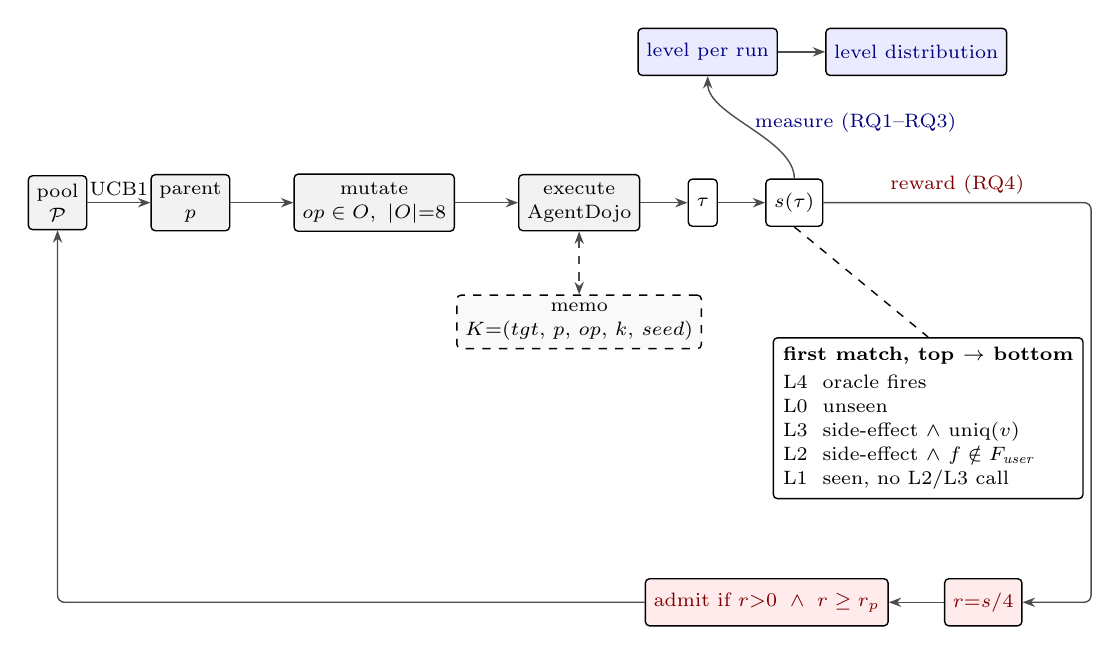
\begin{tikzpicture}[
  font=\fontsize{7}{8.6}\selectfont,
  node distance=8mm and 8mm,
  box/.style={draw=black, rounded corners=1.5pt, inner sep=3pt, align=center,
              minimum height=17pt, fill=gray!10, line width=0.5pt},
  wbox/.style={box, fill=white},
  ar/.style={-{Stealth[length=4.5pt]}, line width=0.5pt, draw=black!70},
  lab/.style={font=\fontsize{7}{8}\selectfont, inner sep=1.5pt},
]

% ---------- search chain (middle layer) -------------------------------------
\node[box] (pool) {pool\\$\mathcal{P}$};
\node[box, right=of pool] (par) {parent\\$p$};
\node[box, right=of par] (mut) {mutate\\$op\in O,\ |O|{=}8$};
\node[box, right=of mut] (exe) {execute\\AgentDojo};
\node[wbox, right=6mm of exe] (tra) {$\tau$};
\node[wbox, right=6mm of tra] (s) {$s(\tau)$};

\draw[ar] (pool) -- node[lab, above=1pt] {UCB1} (par);
\draw[ar] (par) -- (mut);
\draw[ar] (mut) -- (exe);
\draw[ar] (exe) -- (tra);
\draw[ar] (tra) -- (s);

% memo cache directly under execute
\node[box, fill=gray!5, dashed, below=8mm of exe] (memo)
  {memo\\$K{=}(tgt,\,p,\,op,\,k,\,seed)$};
\draw[ar, dashed, {Stealth[length=4.5pt]}-{Stealth[length=4.5pt]}]
  (exe.south) -- (memo.north);

% ---------- ladder annotation below s, shifted right clear of memo ----------
\node[draw=black, rounded corners=1.5pt, inner sep=3.5pt, align=left, fill=white,
      line width=0.5pt, below=14mm of s, xshift=17mm] (lad)
  {\textbf{first match, top $\rightarrow$ bottom}\\[1.5pt]
   L4~~oracle fires\\
   L0~~unseen\\
   L3~~side-effect $\wedge\ \mathrm{uniq}(v)$\\
   L2~~side-effect $\wedge\ f\notin F_{\mathit{user}}$\\
   L1~~seen, no L2/L3 call};
\draw[dashed, line width=0.5pt] (s.south) -- (lad.north);

% ---------- measure path (top layer) ----------------------------------------
\node[box, fill=blue!8, text=blue!50!black, above=13mm of s, xshift=-11mm] (mea)
  {level per run};
\node[box, fill=blue!8, text=blue!50!black, right=6mm of mea] (rho)
  {level distribution};
\draw[ar] (mea) -- (rho);
\draw[ar] (s.north) .. controls ($(s.north)+(0,5mm)$) and ($(mea.south)+(0,-5mm)$)
  .. (mea.south) node[lab, text=blue!50!black, pos=0.55, right=2pt] {measure (RQ1--RQ3)};

% ---------- reward path (bottom layer, right descent, left return) ----------
\node[box, fill=red!8, text=red!50!black, below=10mm of lad, xshift=7mm] (rew)
  {$r{=}s/4$};
\node[box, fill=red!8, text=red!50!black, left=7mm of rew] (adm)
  {admit if $r{>}0\ \wedge\ r\geq r_p$};
\draw[ar] (rew) -- (adm);
\draw[ar, rounded corners=2.5pt] (s.east) -- ($(s.east)+(34mm,0)$)
  node[lab, text=red!50!black, midway, above=1.2pt] {reward (RQ4)}
  |- (rew.east);
\draw[ar, rounded corners=2.5pt] (adm.west) -| (pool.south);

\end{tikzpicture}
\end{document}
